\documentclass{standalone}
\usepackage{tikz}
\begin{document}
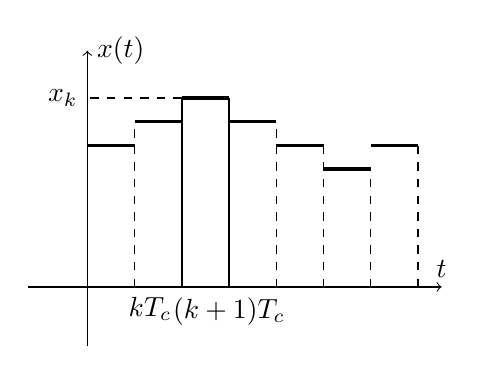
\begin{tikzpicture}[scale=3]
    \draw[->](-0.25,0)--(1.5,0)node[above]{$t$};
    \draw[->](0,-0.25)--(0,1)node[right]{$x(t)$};

    \draw[-,very thick](0,0.6)--(0.2,0.6);
    \draw[-,very thick](0.2,0.7)--(0.4,0.7);
    \draw[-,very thick](0.4,0.8)--(0.6,0.8);
    \draw[-,very thick](0.6,0.7)--(0.8,0.7);
    \draw[-,very thick](0.8,0.6)--(1,0.6);
    \draw[-,very thick](1,0.5)--(1.2,0.5);
    \draw[-,very thick](1.2,0.6)--(1.4,0.6);

    \draw[-, thick](0.4,0.8)--(0.4,0)node[below left]{$kT_c$};        
    \draw[-, thick](0.6,0.8)--(0.6,0)node[below]{$(k+1)T_c$};
    \draw[dashed](0.4,0.8)--(0,0.8)node[left]{$x_k$};
    \draw[dashed](0.2,0)--(0.2,0.7);
    \draw[dashed](0.8,0)--(0.8,0.7);
    \draw[dashed](1,0)--(1,0.6);
    \draw[dashed](1.2,0)--(1.2,0.5);
    \draw[dashed](1.4,0)--(1.4,0.6);
\end{tikzpicture}
\end{document}